% =====================================================================
\appendix

\section{Additional Cross-Validation Results} \label{a:cv}

All results in this appendix come from the same 50 cross-validation runs as Section~\ref{s:results} (5 folds $\times$ 5 models $\times$ 2 directions) unless stated otherwise.

\subsection{All Metrics at a Glance}

\begin{figure*}[t]
	\centering
	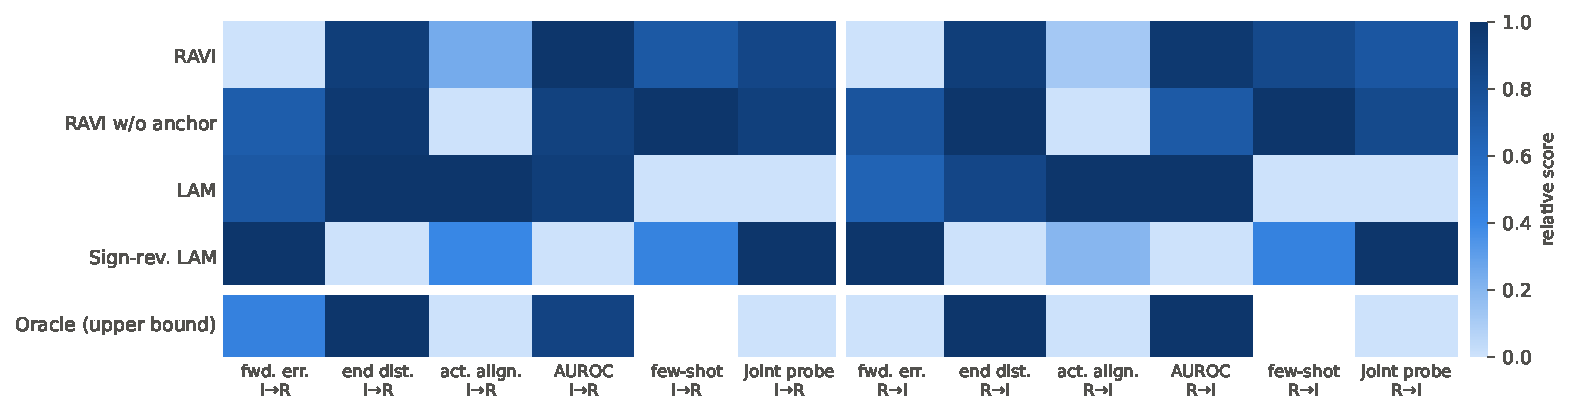
\includegraphics[width=0.92\textwidth]{figs/fig_scorecard_heatmap.pdf}
	\caption{All metrics for all models and both directions. Cells show raw means over 5 folds; shading is scaled per column among the four non-oracle models, so small absolute gaps can look large.}
	\label{f:scorecard}
\end{figure*}

Fig.~\ref{f:scorecard} shows that no model wins everywhere.
The {\method} variants lead on reversibility detection, end distance for R$\to$I and transfer; the plain LAM leads on action alignment and on end distance for I$\to$R; and the sign-reversal LAM has the lowest joint-probe error despite its divergent rollouts.
No model recovers the real reverse joint motion: every probe error exceeds 1.0, although all beat negated, time-reversed joint deltas, which confirms that removal is not insertion played backward.

\subsection{Few-Shot Adaptation at Every $k$}

\begin{table*}
	\centering
	\caption{Opposite-task forward error after fine-tuning only the IDM on $k$ episodes of the opposite task, mean $\pm$ standard deviation over 5 folds. Errors are relative to predicting no change. Best value per column in bold.}
	\label{t:fewshot}
	\footnotesize
	\setlength{\tabcolsep}{4pt}
	\begin{tabular}{lcccccccc}
		\toprule
		& \multicolumn{4}{c}{I$\to$R} & \multicolumn{4}{c}{R$\to$I} \\
		\cmidrule(r){2-5} \cmidrule(l){6-9}
		Model & $k=0$ & $k=1$ & $k=3$ & $k=5$ & $k=0$ & $k=1$ & $k=3$ & $k=5$ \\
		\midrule
		LAM & 1.136$\pm$0.035 & 1.115$\pm$0.029 & 1.101$\pm$0.027 & 1.099$\pm$0.026 & 0.911$\pm$0.032 & 0.892$\pm$0.023 & 0.878$\pm$0.024 & 0.872$\pm$0.024 \\
		Sign-rev. LAM & 1.090$\pm$0.030 & 1.078$\pm$0.021 & 1.064$\pm$0.021 & 1.060$\pm$0.021 & 0.870$\pm$0.029 & 0.865$\pm$0.029 & 0.846$\pm$0.027 & 0.840$\pm$0.027 \\
		{\method} w/o anchor & \textbf{1.034}$\pm$0.029 & \textbf{1.020}$\pm$0.020 & \textbf{1.011}$\pm$0.017 & \textbf{1.008}$\pm$0.019 & \textbf{0.821}$\pm$0.033 & \textbf{0.818}$\pm$0.031 & \textbf{0.801}$\pm$0.030 & \textbf{0.796}$\pm$0.030 \\
		{\method} & 1.062$\pm$0.030 & 1.056$\pm$0.024 & 1.037$\pm$0.025 & 1.033$\pm$0.023 & 0.837$\pm$0.032 & 0.840$\pm$0.022 & 0.813$\pm$0.025 & 0.808$\pm$0.026 \\
		\bottomrule
	\end{tabular}
\end{table*}

Table~\ref{t:fewshot} lists the few-shot errors behind Fig.~\ref{f:fewshot}.
The two {\method} variants are the two best models at every $k$ in both directions, and the gap to the LAM baselines is present already at $k=0$, before any adaptation.

\subsection{Reference Values}
Negated, time-reversed joint deltas of the paired forward episode reach a joint-probe error of $1.583\pm0.090$ for I$\to$R and $1.533\pm0.044$ for R$\to$I, worse than every learned model in Table~\ref{t:main}.
Stage reach is noisy with 10 test episodes per fold (Table~\ref{t:main}); the end-distance ratio is the more stable rollout measure.

\subsection{Per-Fold Results}
Tables~\ref{t:perfoldI} and~\ref{t:perfoldR} give the per-fold values of the main reverse-direction metrics.
The sign-reversal LAM has an end-distance ratio above 1.29 in every fold of both directions, while every Koopman model stays below 1.0 in every fold.

\begin{table*}
\centering
\caption{Per-fold results, trained on insertion, tested on removal (I$\to$R). Folds are disjoint sets of test episodes.}
\label{t:perfoldI}
\footnotesize
\setlength{\tabcolsep}{4pt}
\begin{tabular}{llccccc}
\toprule
Metric & Model & Fold 0 & Fold 1 & Fold 2 & Fold 3 & Fold 4 \\
\midrule
\multirow{5}{*}{End-distance ratio $\downarrow$} & LAM & 0.611 & 0.696 & 0.785 & 0.789 & 0.662 \\
 & Sign-rev. LAM & 1.694 & 1.573 & 1.296 & 1.783 & 1.415 \\
 & \method{} w/o anchor & 0.790 & 0.779 & 0.736 & 0.716 & 0.660 \\
 & \method & 0.783 & 0.725 & 0.752 & 0.873 & 0.710 \\
 & Oracle & 0.697 & 0.666 & 0.642 & 0.756 & 0.747 \\
\midrule
\multirow{5}{*}{Reversibility AUROC $\uparrow$} & LAM & 0.795 & 0.710 & 0.695 & 0.801 & 0.685 \\
 & Sign-rev. LAM & 0.670 & 0.647 & 0.400 & 0.790 & 0.542 \\
 & \method{} w/o anchor & 0.752 & 0.753 & 0.725 & 0.777 & 0.656 \\
 & \method & 0.767 & 0.768 & 0.730 & 0.794 & 0.673 \\
 & Oracle & 0.740 & 0.772 & 0.696 & 0.758 & 0.691 \\
\midrule
\multirow{5}{*}{Action alignment $\uparrow$} & LAM & 0.181 & 0.161 & 0.207 & 0.172 & 0.163 \\
 & Sign-rev. LAM & 0.146 & 0.125 & 0.153 & 0.141 & 0.132 \\
 & \method{} w/o anchor & 0.121 & 0.098 & 0.124 & 0.120 & 0.110 \\
 & \method & 0.139 & 0.113 & 0.143 & 0.130 & 0.125 \\
 & Oracle & 0.106 & 0.194 & 0.077 & 0.102 & 0.052 \\
\midrule
\multirow{4}{*}{Few-shot error, $k=5$ $\downarrow$} & LAM & 1.088 & 1.094 & 1.065 & 1.144 & 1.106 \\
 & Sign-rev. LAM & 1.071 & 1.056 & 1.021 & 1.076 & 1.076 \\
 & \method{} w/o anchor & 1.004 & 1.015 & 0.976 & 1.033 & 1.011 \\
 & \method & 1.046 & 1.035 & 0.993 & 1.062 & 1.030 \\
\bottomrule
\end{tabular}
\end{table*}

\begin{table*}
\centering
\caption{Per-fold results, trained on removal, tested on insertion (R$\to$I). Folds are disjoint sets of test episodes.}
\label{t:perfoldR}
\footnotesize
\setlength{\tabcolsep}{4pt}
\begin{tabular}{llccccc}
\toprule
Metric & Model & Fold 0 & Fold 1 & Fold 2 & Fold 3 & Fold 4 \\
\midrule
\multirow{5}{*}{End-distance ratio $\downarrow$} & LAM & 0.948 & 0.905 & 0.911 & 0.962 & 0.830 \\
 & Sign-rev. LAM & 1.817 & 2.135 & 1.483 & 2.052 & 1.811 \\
 & \method{} w/o anchor & 0.714 & 0.802 & 0.796 & 0.767 & 0.750 \\
 & \method & 0.853 & 0.815 & 0.839 & 0.741 & 0.962 \\
 & Oracle & 0.588 & 0.594 & 0.594 & 0.627 & 0.615 \\
\midrule
\multirow{5}{*}{Reversibility AUROC $\uparrow$} & LAM & 0.554 & 0.570 & 0.593 & 0.792 & 0.692 \\
 & Sign-rev. LAM & 0.304 & 0.510 & 0.459 & 0.292 & 0.456 \\
 & \method{} w/o anchor & 0.524 & 0.535 & 0.635 & 0.590 & 0.586 \\
 & \method & 0.576 & 0.590 & 0.689 & 0.635 & 0.678 \\
 & Oracle & 0.611 & 0.630 & 0.724 & 0.691 & 0.663 \\
\midrule
\multirow{5}{*}{Action alignment $\uparrow$} & LAM & 0.230 & 0.235 & 0.268 & 0.228 & 0.241 \\
 & Sign-rev. LAM & 0.153 & 0.146 & 0.161 & 0.140 & 0.163 \\
 & \method{} w/o anchor & 0.124 & 0.119 & 0.143 & 0.126 & 0.142 \\
 & \method & 0.140 & 0.125 & 0.149 & 0.143 & 0.162 \\
 & Oracle & 0.100 & 0.189 & 0.049 & 0.097 & 0.044 \\
\midrule
\multirow{4}{*}{Few-shot error, $k=5$ $\downarrow$} & LAM & 0.918 & 0.851 & 0.875 & 0.860 & 0.857 \\
 & Sign-rev. LAM & 0.885 & 0.808 & 0.828 & 0.852 & 0.824 \\
 & \method{} w/o anchor & 0.825 & 0.744 & 0.790 & 0.823 & 0.802 \\
 & \method & 0.831 & 0.770 & 0.789 & 0.840 & 0.811 \\
\bottomrule
\end{tabular}
\end{table*}


\subsection{Walkthrough of the Model Variables}

\begin{figure*}[t]
	\centering
	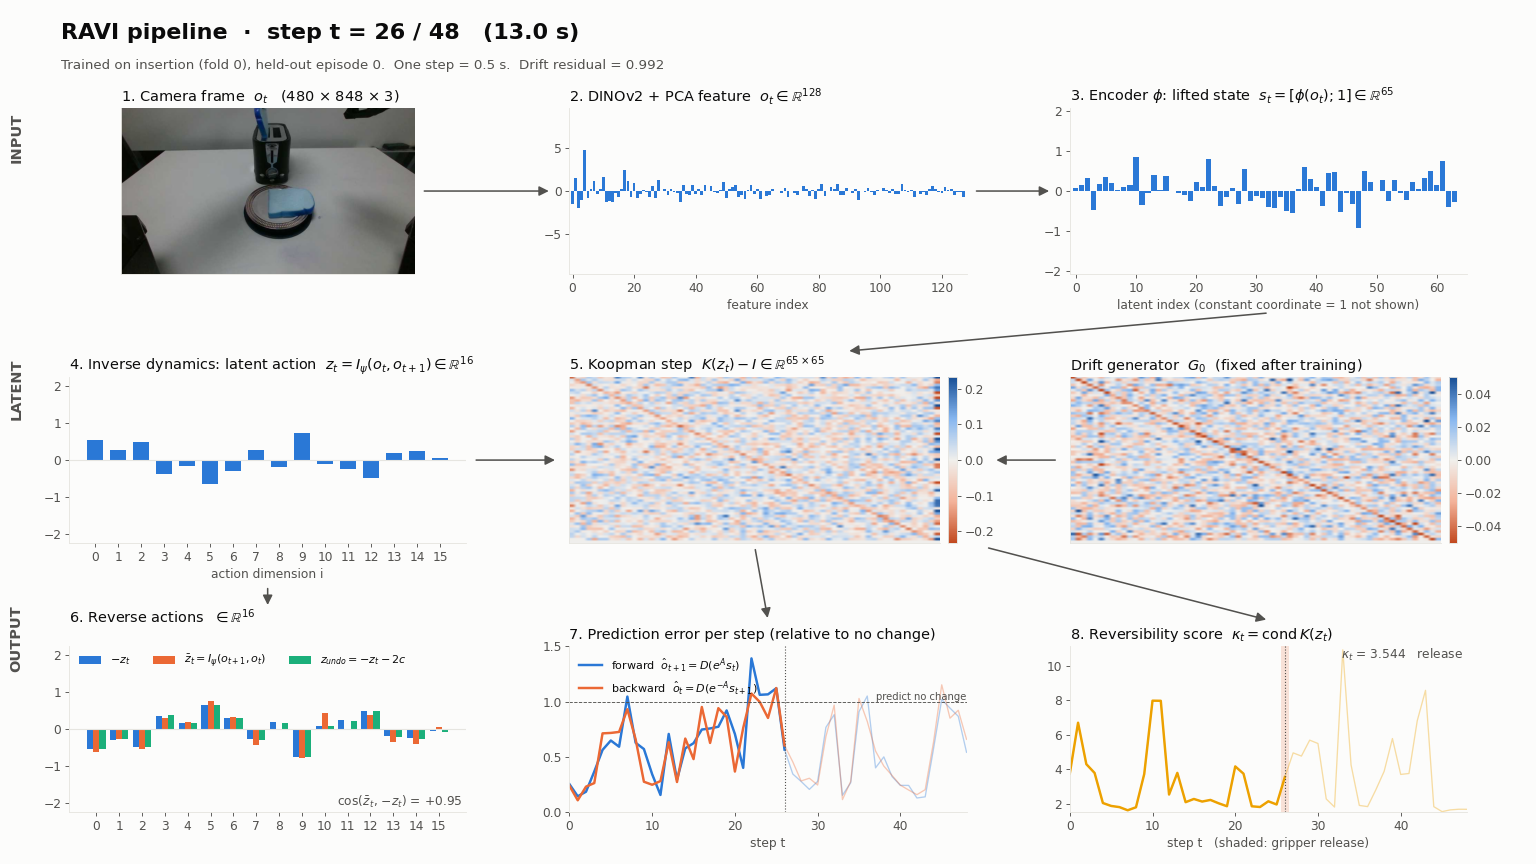
\includegraphics[width=\textwidth]{figs/fig_walkthrough.png}
	\caption{All {\method} variables at step 26 of a held-out insertion episode (13.0\,s, the first release): camera frame, feature $o_t$, lifted state $s_t$, latent action $z_t$, step operator $K(z_t)-I$, drift $G_0$, reverse actions, prediction errors and the reversibility score $\kappa_t$. A video of all 49 steps accompanies the paper.}
	\label{f:walk}
\end{figure*}

Fig.~\ref{f:walk} shows every variable of a model trained on insertion (fold 0), on a held-out insertion episode.
Reversal consistency is strong: the IDM output on the swapped pair nearly mirrors $-z_t$ (cosine $+0.95$ at the release step).
Because the drift residual is 0.992 for this model, $\zundo$ is almost identical to $-z_t$, in line with Proposition~\ref{p:undo}(c).
In this episode $\kappa_t$ does not peak at the release itself (step 26, $\kappa_t=3.5$); its largest values occur at steps 10, 33 and 43, likely other contact events.
The AUROC of Table~\ref{t:main} is an aggregate over many episodes, and single episodes can be noisier.

% =====================================================================
\section{Controlled Study with Known Drift} \label{a:toy}

\begin{table}
	\centering
	\caption{Two-dimensional point with constant drift $g$, observed through a random nonlinear lift. The analytic undo action is $u'=-u-2g$. Return error is the simulator distance to $p_t$ after executing the undo action, divided by the step length.}
	\label{t:toy}
	\footnotesize
	\setlength{\tabcolsep}{4pt}
	\begin{tabular}{lcc}
		\toprule
		Quantity & No reversal loss & Reversal loss \\
		\midrule
		Forward relative error & 0.023 & 0.013 \\
		Backward relative error (never trained) & 0.012 & 0.009 \\
		$\cos(\text{IDM}(o_{t+1},o_t),-z)$ & 0.62 & 0.995 \\
		No-op code size $\|z_{\text{no-op}}\|/\mathrm{rms}(z)$ & 0.36 & 0.48 \\
		Linear probe $R^2$, $z\to u$ & 0.84 & 0.89 \\
		Return error, model undo action & 0.34 & 0.26 \\
		Return error, naive $u'=-u$ & 1.15 & 1.15 \\
		Mean $|u_{\text{undo}}-(-u-2g)|$ (naive: 0.5) & 0.19 & 0.15 \\
		\bottomrule
	\end{tabular}
\end{table}

To test the theory where the ground truth is known, we simulate a two-dimensional point $p_{t+1}=p_t+\Delta t\,(g+u)$ with constant drift $g=(0,-0.5)$, actions $u\in[-1,1]^2$ and $\Delta t=0.1$, observed only through a fixed random two-layer $\tanh$ lift to 32 dimensions.
A Koopman model with $d=8$, $m=2$ and a constant coordinate is trained for 6,000 steps on forward transitions only, once without and once with the reversal-consistency loss (Table~\ref{t:toy}).
Errors are relative to predicting no change and evaluated on 8,000 fresh transitions.
\begin{itemize}
	\item Backward prediction through the exact inverse is as accurate as forward prediction although it is never trained, as Proposition~\ref{p:inverse} predicts.
	\item The IDM is not reversal-consistent by itself (cosine 0.62); the reversal loss makes it so (0.995) and, without an anchor, moves part of the drift into the latent code (no-op code size 0.48), as Proposition~\ref{p:gauge} allows.
	\item The undo action is found by planning in the model, mapped to real actions with a linear probe fitted on labeled transitions (which fixes the gauge), and executed in the simulator. It returns the point to within 0.26--0.34 step lengths, whereas naively negating the action misses by 1.15, and the recovered action is close to the analytic $-u-2g$. The remaining error tracks the probe $R^2$ of 0.84--0.89.
\end{itemize}

% =====================================================================
\section{Development Runs} \label{a:dev}

The runs in this appendix were made while designing the evaluation, on insertion, fold 0, with one run per setting.
They are not cross-validated and are reported for completeness.
Where marked, the reversibility AUROC used an earlier release rule that counted gripper openings without a prior hold; that rule fired 3--5 times per episode and was replaced by the rule in Section~\ref{s:setup}, so those AUROC values are not comparable with Table~\ref{t:main}.

\begin{table*}
	\centering
	\caption{Development runs (insertion, fold 0, one run each). Errors are relative to predicting no change. $^\dagger$AUROC with the earlier release rule (not comparable with Table~\ref{t:main}).}
	\label{t:dev}
	\footnotesize
	\setlength{\tabcolsep}{4pt}
	\begin{tabular}{llcccccc}
		\toprule
		Setting & Model & Forward err. & Backward err. & End dist. & Action align. & Joint probe & AUROC \\
		\midrule
		\multirow{4}{*}{Step 0.1\,s} & Sign-rev. LAM & 0.508 & 0.512 & $7.5\times10^5$ & 0.063 & 0.981 & 0.379$^\dagger$ \\
		& {\method} w/o anchor & 0.525 & 0.525 & 1.033 & 0.058 & 0.975 & 0.460$^\dagger$ \\
		& {\method} & 0.538 & 0.540 & 0.981 & 0.056 & 0.982 & 0.426$^\dagger$ \\
		& Oracle & 0.521 & 0.522 & 0.851 & 0.032 & 1.048 & 0.436$^\dagger$ \\
		\midrule
		\multirow{4}{*}{Step 0.5\,s} & Sign-rev. LAM & 0.227 & 0.231 & 1.477 & 0.140 & 1.010 & 0.370$^\dagger$ \\
		& {\method} w/o anchor & 0.230 & 0.235 & 0.959 & 0.116 & 1.051 & 0.482$^\dagger$ \\
		& {\method} & 0.235 & 0.241 & 1.049 & 0.137 & 1.047 & 0.472$^\dagger$ \\
		& Oracle & 0.232 & 0.233 & 0.734 & 0.086 & 1.280 & 0.473$^\dagger$ \\
		\midrule
		\multirow{3}{*}{\shortstack[l]{Step 0.5\,s,\\new release rule}} & LAM & 0.231 & 0.232 & 0.684 & 0.208 & 1.147 & 0.580 \\
		& {\method}, $\lambda_v=10^{-5}$ & 0.239 & 0.243 & 1.345 & 0.117 & 1.047 & 0.711 \\
		& {\method}, $\lambda_v=0$ & 0.239 & 0.244 & 1.389 & 0.117 & 1.046 & 0.711 \\
		\bottomrule
	\end{tabular}
\end{table*}

\paragraph{Step size.}
A step of 0.1\,s left forward error at about 0.5 of the no-change baseline for every model, because consecutive frames barely differ, and the sign-reversal LAM's rollout diverged by five orders of magnitude (Table~\ref{t:dev}).
A step of 0.5\,s, trained on all five phase offsets, halved the error, and we use it throughout.

\paragraph{Symmetric action blocks.}
Weakening the penalty on the symmetric action blocks ($\lambda_v=10^{-5}$ or 0) left every metric and the drift residual (0.992) essentially unchanged.
The residual therefore does not come from the penalty, which led us to fit $c$ on visited states.

\paragraph{Fitting the drift-equivalent action.}
Fitting $c$ on whole matrices, $\min_c\|G_0-\sum_ic_iG_i\|_F$, gave a residual of 0.991 on this fold; fitting on visited states, Eq.~(\ref{e:undo}), gives $0.988\pm0.005$ across folds.
Both are near 1 because 16 action generators cannot cancel the drift's effect in a 65-D lifted space.

\paragraph{Release labels.}
With a hold requirement of 1\,s before a gripper opening past 0.9, exactly two releases are found in 41 of 50 insertion and 49 of 50 removal episodes, matching the two slices per episode.
Without the hold requirement, most episodes showed 3--5 spurious releases, because the gripper passes through the holding range while opening and closing.

\paragraph{Feature check.}
To rule out the visual representation as the cause of transfer limits, we trained a linear probe (logistic regression on 256 PCA dimensions, 5-fold episode split) to decode the three scene stages from 40 episodes at 2\,Hz, using the release-based stage labels.
Table~\ref{t:feat} shows that every variant decodes the stage almost perfectly, so we keep the top-camera CLS token with a $2\times4$ grid.

\begin{table}
	\centering
	\caption{Stage decoding from features, balanced accuracy over 5 episode folds (chance 0.333).}
	\label{t:feat}
	\footnotesize
	\begin{tabular}{lc}
		\toprule
		Features & Balanced accuracy \\
		\midrule
		Top camera, CLS + $2\times4$ grid (used) & 0.975$\pm$0.003 \\
		Top camera, CLS + $4\times7$ grid & 0.979$\pm$0.002 \\
		Wrist cameras, CLS + $2\times4$ grid & 0.982$\pm$0.009 \\
		Top $4\times7$ + wrists & 0.984$\pm$0.003 \\
		\bottomrule
	\end{tabular}
\end{table}

% =====================================================================
\section{Implementation Details} \label{a:impl}

All models share the following settings.
\begin{itemize}
	\item \textbf{Input:} top camera, $480\times848$, resized to $224\times392$; frozen DINOv2 ViT-S/14; CLS token (384) and a $2\times4$ pooled patch grid (3,072), standardised and reduced by PCA to 128 dimensions with unit average variance.
	\item \textbf{Networks:} head $\phi$ and decoder are MLPs with two hidden layers of 256 units and GELU; the IDM is an MLP on $[o_t,o_{t+1},o_{t+1}-o_t]$ (384 inputs, 16 outputs).
	\item \textbf{Latents:} $d=64$ plus the constant coordinate; $m=16$, with Gaussian noise of 0.05 on $z$ during training.
	\item \textbf{Data:} one step is 0.5\,s (5 frames at 10\,Hz), using all 5 phase offsets for training; the anchor set is the slowest 15\% of steps by joint speed.
	\item \textbf{Optimisation:} Adam, learning rate $10^{-3}$, batch 512, 4,000 steps; $\lambda_b=\lambda_r=\lambda_a=1$, $\lambda_v=10^{-3}$; $c$ is fitted on 2,000 training latents; few-shot adaptation uses 500 IDM steps with batch 256.
	\item \textbf{Compute:} one A100 80\,GB GPU, about 10 minutes per run.
\end{itemize}
LAM baselines use MLP forward and backward models with the same hidden sizes; their reversibility score is the condition number of the forward-model Jacobian with respect to the lifted state.
The 50 cross-validation runs were scheduled two to three at a time to respect the GPU quota of the shared server.
Code, per-fold results and the walkthrough video are released with the paper.
